\documentclass{article}
\usepackage[utf8]{inputenc}
\usepackage{graphicx} 
\usepackage{amsmath} 
\setlength{\parindent}{4em}
\setlength{\parskip}{1em}
\renewcommand{\baselinestretch}{1.5}
\newcommand{\Tau}{\mathrm{T}}

\title{BLG 354E Homework - 3}
\author{Yunus Güngör }
\date{May 2018}

\begin{document}
	
	\maketitle
	
	\section{Answers}
	
	This homework only includes answers to given questions
	
	1)\par
	a)This system is not casual due to output depending on a value at $t+2$
	This system is not stable since $d(x)/dt$ is not bounded if $|x(t)|<B_x$ 
	\par 
	b)This system is casual since output does not depend any future value at $t+n$
	This system is stable because it can be bounded, if $x$ is also bounded.
	\par 
	c)This system is casual since output does not depend any future value at $t+n$
	$$\int_{-\infty}^{\inf}e^{-(t-5)}u(t-5)=\int_{t=5}^{\infty}e^{-(t-5)}=-e^{5-t}=-e^5/e^t$$
	$$lim_{t\rightarrow \infty}-e^5/e^t=0$$
	$$-e^5/e^t<0$$
	This system can be bounded therefore it is stable
	\par 
	d)This system is casual since output does not depend any future value at $t+n$
	$$\int_{t=-\infty}^{\infty}u(t)-e^{-3t}u(t)=\int_{t=0}^{\infty}1-e^{-3t}=1+e^{\infty}-2=\infty$$
	This system can not be bounded therefore it is not stable
	\par
	
	2)
	$$\int_{-\infty}^{\infty}5e^{-0.5(t-\Tau-3)}[u(t-\Tau-3)-u(t-\Tau-11)] u(\Tau-2) d\Tau=$$\par
	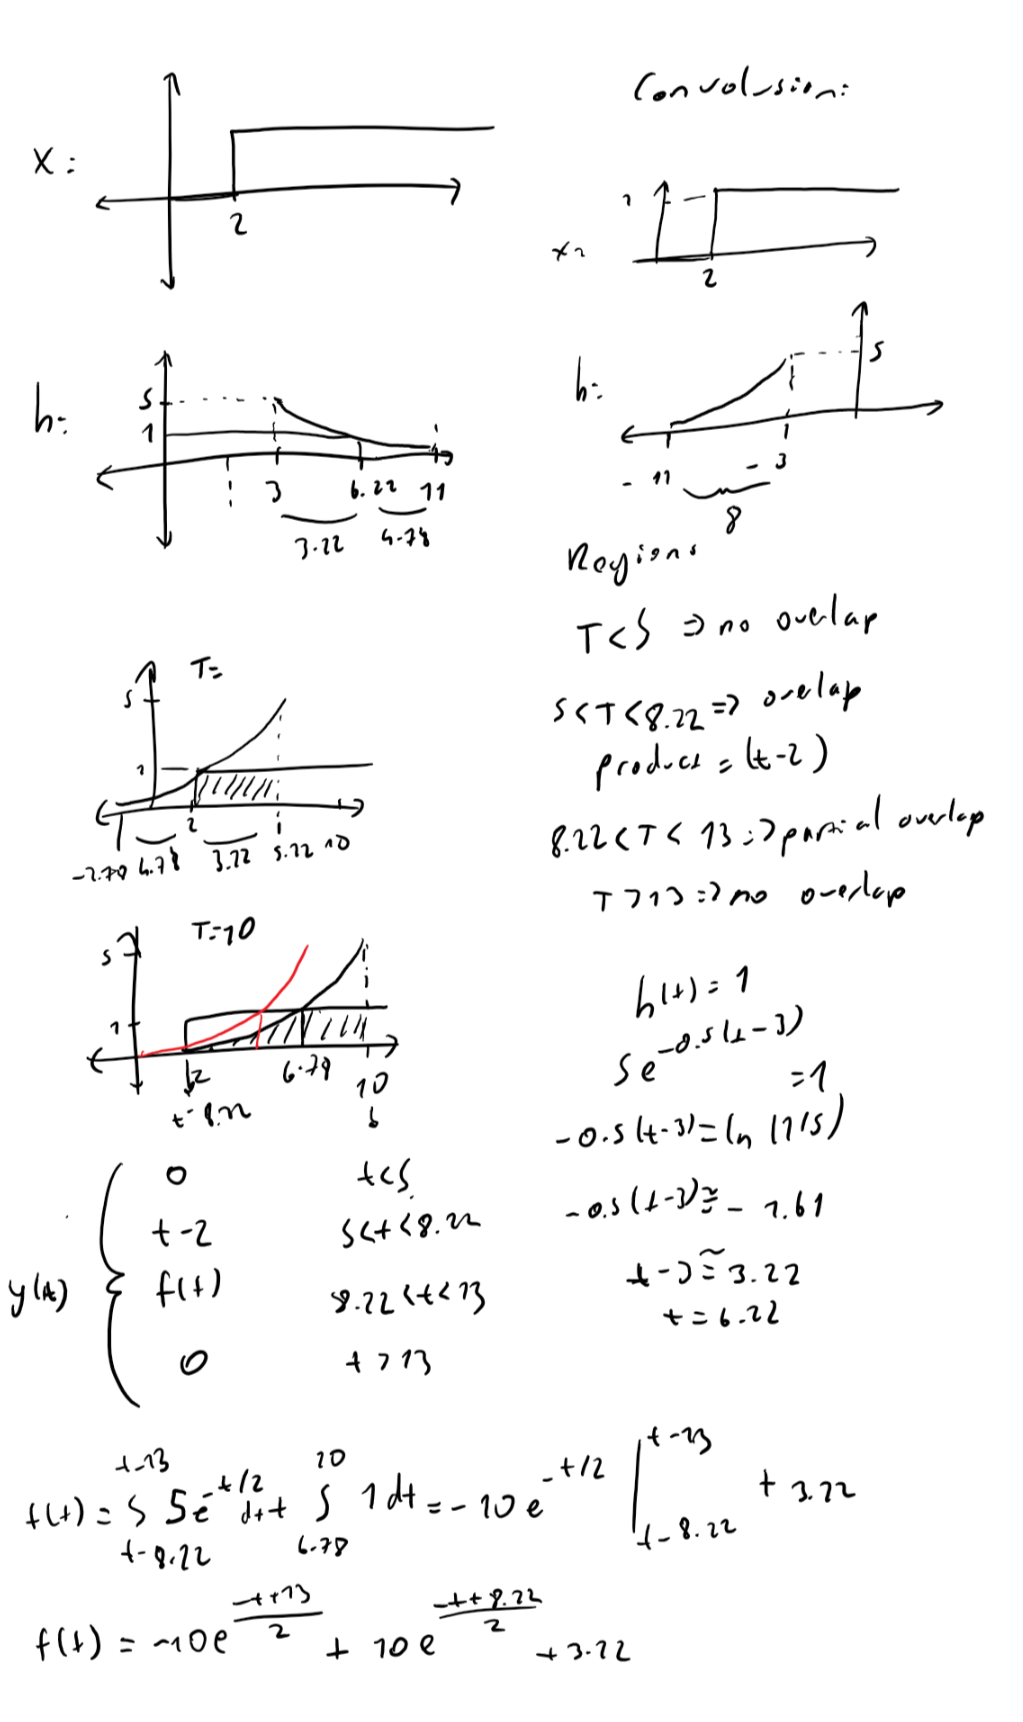
\includegraphics[scale=0.7]{q2}	\par
	3)You can find solution in attached files
	\par
	4)Code for this question can be found in attachment.\par
	Result:\par
	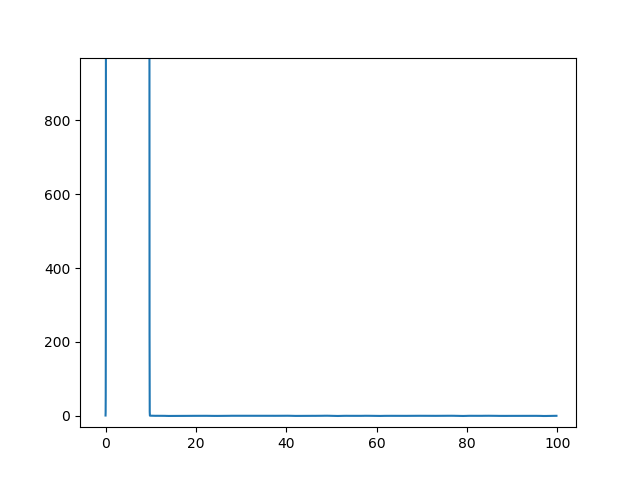
\includegraphics[scale=0.7]{q4}\par
	Results have infite value for $0<t<1$	
	\par
	 5)\par
	 a)
	 $$H(jw)=\int^{\infty}_{-\infty}h(t)e^{-jwt}dt$$
	 $$H(jw)=\int^{\infty}_{-\infty} (\delta(t-2)-0.2e^{-0.2(t-2)}[u(t-2)])e^{-jwt}dt$$
	 $$\int^{\infty}_{-\infty}\delta(t-2)e^{-jwt}dt - 0.2 \int^{\infty}_{-\infty}u(t-2)e^{-jwt-0.2(t-2)}dt $$
	 $$e^{-2jw}-0.2\int^{\infty}_{2}e^{-jwt-0.2(t-2)}dt $$
	 $$e^{-2jw}-0.2\int^{\infty}_{2}e^{(-jw-0.2)t-0.4)}dt$$
	 $$H(jw)=e^{-2jw}-0.2 \frac{e^{2jw}}{jw+0.2}$$

	 \par
	 b)
	 $$|H(jw)|^2=H(jw)H^*(jw)$$
	 $$=(e^{-2jw}-0.2 \frac{e^{2jw}}{jw+0.2})(e^{2jw}-0.2 \frac{e^{-2jw}}{-jw+0.2})$$
	 $$=1-0.2 \frac{e^{4jw}}{jw+0.2}+0.2 \frac{e^{-4jw}}{jw-0.2}+0.04\frac{1}{w^2+0.04}$$
	 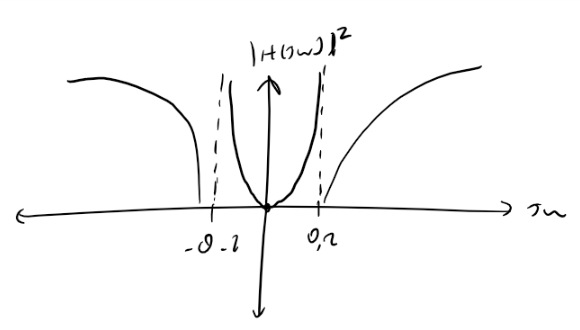
\includegraphics[scale=0.7]{q5b}\par
	 
	 c)\par 
	 $$y(t)=h(t)x(t)$$
	 $$x(t)=ax_1(t)+bx_2(t)$$
	 $$y_1(t)=h(t)x_1(t)$$
	 $$ y_2(t)=h(t)x_1(t) $$
	 $$y(t)=ay_1(t)+by_2(t)$$
	 \par 
	 
	 6)\par 
	 a)
	 $$\frac{1}{2\pi} \int_{-\infty}^{\infty} \frac{sin(10w)^2}{2w^2}e^{iwt}dw$$
	 b)
	 $$\frac{1}{2\pi} \int_{-\infty}^{\infty} \frac{1}{25+w^2}e^{iwt}dw$$
	 c)
	 $$\int_{-\infty}^{\infty} e^{-a(t-w)}u(t-2)cos(w_0 t)e^{iwt}dt$$
	  
	\par
\end{document}